\documentclass[14pt]{report}
\usepackage{mathtext}
\usepackage{bm}
\usepackage{amssymb}
\usepackage{xcolor}
% \usepackage[T2A]{fontenc}
\usepackage[unicode]{hyperref}
\usepackage[utf8]{inputenc}
\usepackage[14pt]{extsizes}
\usepackage[english, russian]{babel}
\usepackage{indentfirst}
\usepackage{wasysym}
\usepackage{latexsym}
\definecolor{linkcolor}{rgb}{0.0,0.0,0.0}
\definecolor{urlcolor}{HTML}{799B03}
\hypersetup{pdfstartview=FitH, linkcolor=linkcolor,urlcolor=urlcolor, colorlinks=true}
\usepackage{float}
\usepackage[
    left=30mm,
    top=20mm,
    right=10mm,
    bottom=20mm
]{geometry}
\usepackage{euscript}
\usepackage{graphicx}
\usepackage{subcaption}
\usepackage{float}
\usepackage{listings}
\usepackage{csquotes}
\usepackage{mathrsfs}
\usepackage{amssymb}
\usepackage{caption}
\usepackage{titlesec}
%\usepackage[outputdir=output]{minted}
\usepackage{minted}
\graphicspath{ {./images/}{../images/} }

% figure caption type changed
\captionsetup{labelsep=space}
\addto\captionsrussian{\renewcommand{\figurename}{Рисунок}}
% chapter settings
\titleformat{\chapter}[display]
{\centering\Large\bfseries}{\chaptertitlename\ \thechapter}{10pt}{\Large}
\titlespacing*{\chapter}{5pt}{-20pt}{30pt}

% section settings
\titleformat{\section}[block]
  {\large\bfseries}
  {\thesection\ }{0pt}{}

% settings for chapters and sections
\addto\captionsrussian{% Replace "english" with the language you use
  \renewcommand{\contentsname}%
    {\centering \large ОГЛАВЛЕНИЕ}%
  \renewcommand{\chaptername}{ГЛАВА}
  \renewcommand{\chaptertitlename}{ГЛАВА}
  \renewcommand{\bibname}{\large СПИСОК ИСПОЛЬЗОВАННОЙ ЛИТЕРАТУРЫ}
}

\renewcommand{\baselinestretch}{1.2}

\begin{document}

\chapter{Виды нейронных сетей.}

\section{Детерминированные нейронные сети.}

Сначала напомним, что такое обычные(детерминированные) нейронные сети и как они обучаются.

Основная задача обычных искусственных нейронных сетей($ANN$) в том, чтобы аппроксимировать некоторую зависимость выхода $y$ от
 входа $x$: $y = \Phi(x)$. Зависимость $\Phi(x)$ аппроксимируем через композицию последовательных преобразований.

Для простоты будем рассматривать обычные \textit{полносвязные} сети со входом $x$,
 скрытыми(промежуточными) состояниями слоёв $\bm{h_i}$, функциями активации $a_i(\cdot)$ и выходом $y$:
$$\bm{h_0} = \bm{x}$$
$$\bm{h_i} = a_i(\bm{W_i} \cdot h_{i-1} + \bm{b_i}), i = \overline{1...n}$$
$$\bm{h_n} = \widehat{y}$$
$$L = \mathcal{L}(\widehat{y}, y),$$ где $\mathcal{L}(\cdot, \cdot)$ - функция ошибки.

Обозначим параметры модели на $i$-ом слое $\bm{\theta_i} = (\bm{W_i}, \bm{b_i})$, а параметры всей модели через $\bm{\Theta} = \{\bm{\theta_i} :~i~=~\overline{1...n}\}$.
Чаще всего нейронные сети принято рассматривать, как вычислительный граф/граф вычислений.
 Такой подход удобен с инженерной точки зрения, поскольку позволяет воспользоваться инструментом автоматического
 дифференцирования, и используется во всех современных фреймоворках: PyTorch, TensorFlow и прочие.
 Граф вычислений является ациклическим ориентированным графом, составленным из вершин-переменных и вершин-операций(Рисунок \ref{fig:image1}).
\begin{figure}[H]
    \centering
    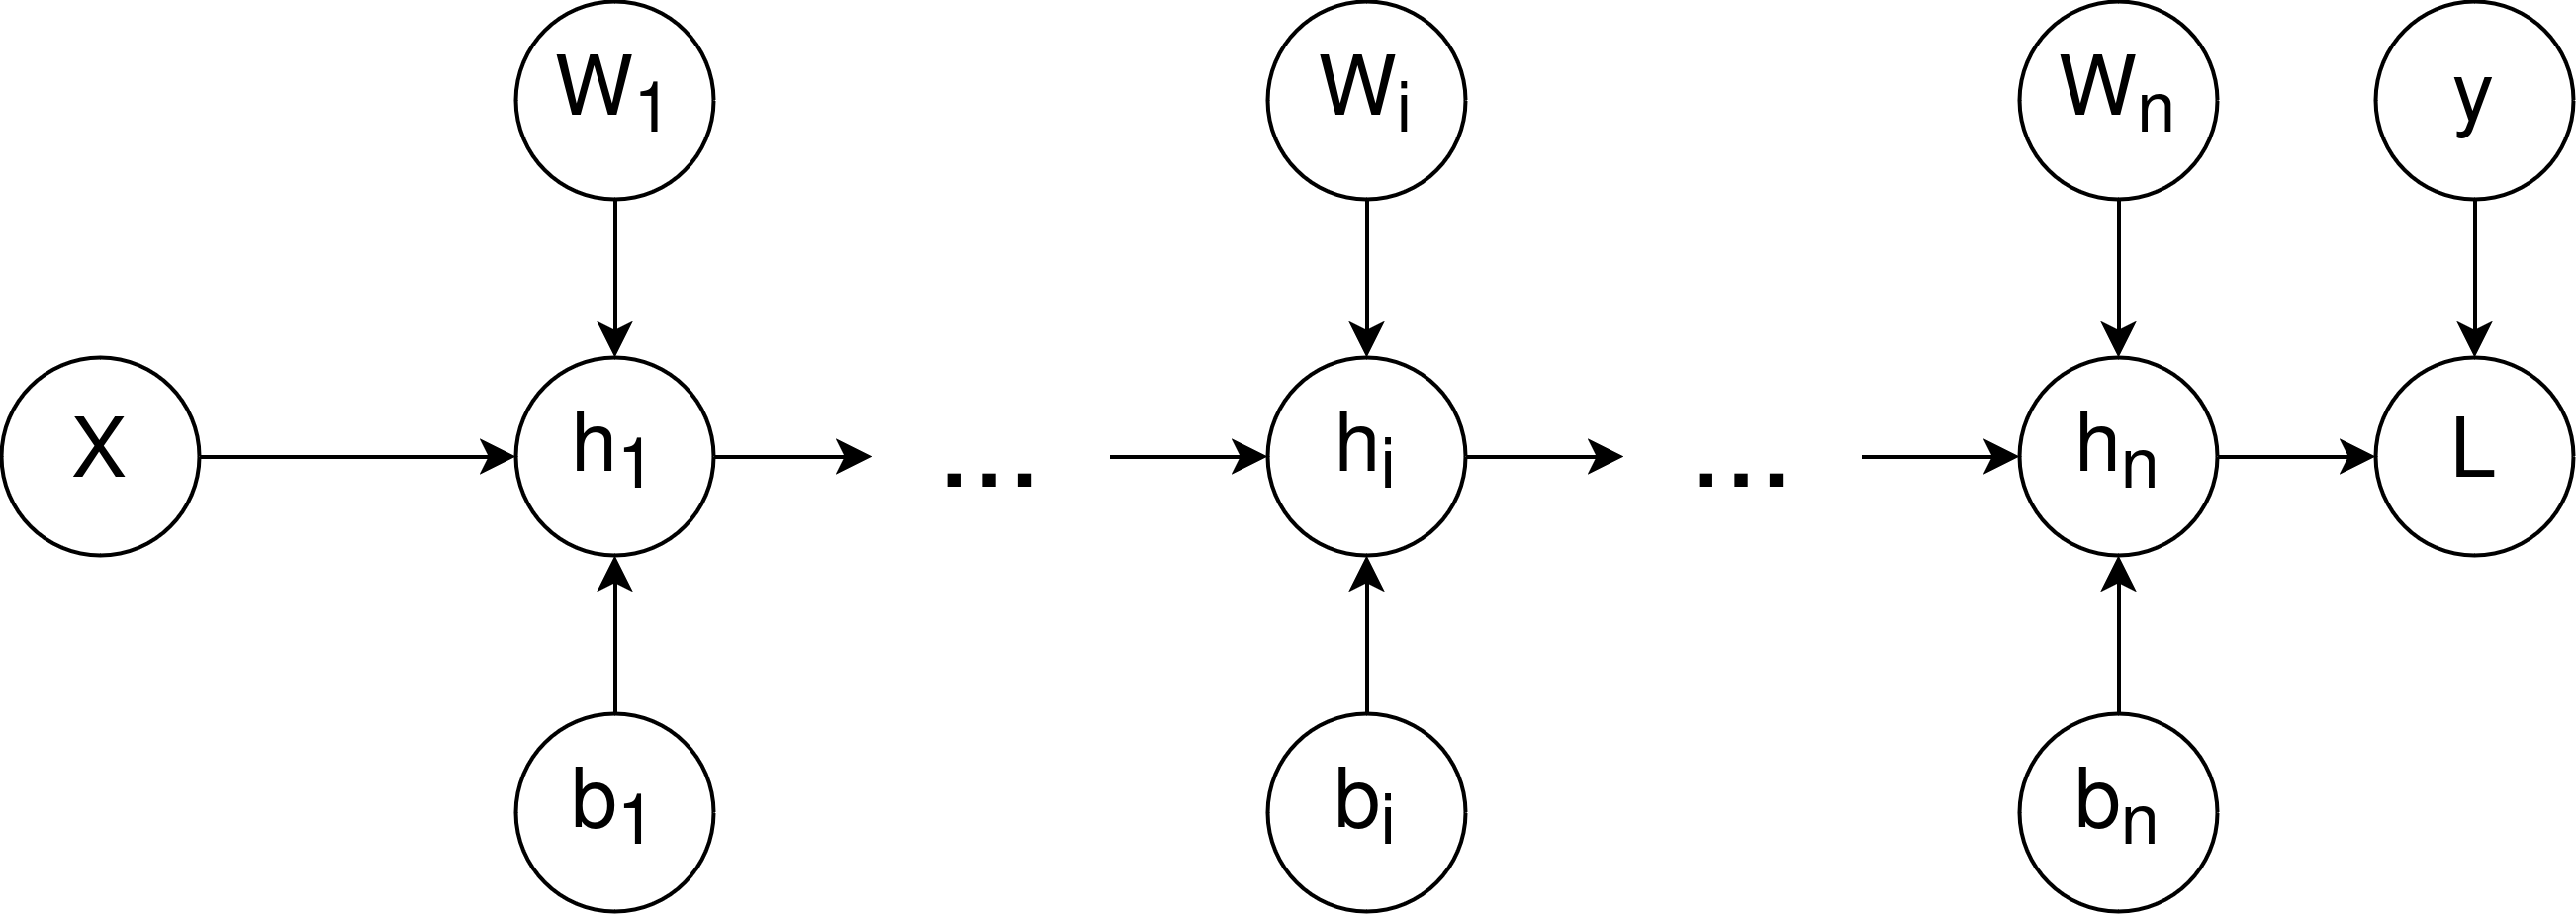
\includegraphics[width=8.5cm]{ANN.png}
    \caption{\textit{Полносвязная} сеть в виде графа вычислений}
    \label{fig:image1}
\end{figure}

Далее будем называть модели, основанные на графах вычислений, --- графовыми моделями. Графы вычислений могут разных типов:
 статическими/динамическими, детерминированными/вероятностными и т.д. Для обучения/настройки параметров детерминированных графовых моделей
 используется метод \textit{обратного распространения ошибки(back propagation)}, который широко используется в современном мире. Вкратце напомним алгоритм:

После прямого выполнения графа(\textit{forward pass}), то есть в соответствии с направлениями рёбер на выходе мы получаем
 $L$ -значение функции ошибки, которые в зависимости от задач мы хотим либо минимизировать, либо максимизировать. Для этого
 мы пользуемся градиентными методами оптимизации, что требует вычисление градиентов $\frac{dL}{d W_i}, \frac{dL}{d b_i}$ по нашим параметрам модели, где $i = \overline{1,n}$.
 В общем случае это трудная задача, однако в случае детерминированных графовых моделей мы можем использовать цепное правило(\textit{chain rule}) для того, чтобы последовательно
 проталкивать градиенты, начиная с концевой вершины, содержащей $L$.

 Например, для подсчёта градиентов $\frac{dL}{d W_i}, \frac{dL}{d b_i}$ мы представим его в виде
 $$\frac{dL}{d W_i} = \frac{dL}{d h_n} \cdot \frac{d h_n}{d W_i}$$
 $$\frac{dL}{d b_i} = \frac{dL}{d h_n} \cdot \frac{d h_n}{d b_i}$$

Аналогично для всех остальных параметров модели мы будем проталкивать накопленный с концевой вершины градиент до соответствующих вершин и
 с помощью этого градиента высчитывать градиент по параметрам модели. Схему работы алгоритма обратного распространения ошибки
 можно увидеть на Рисунок~\ref{fig:image2}.
\begin{figure}[H]
    \centering
    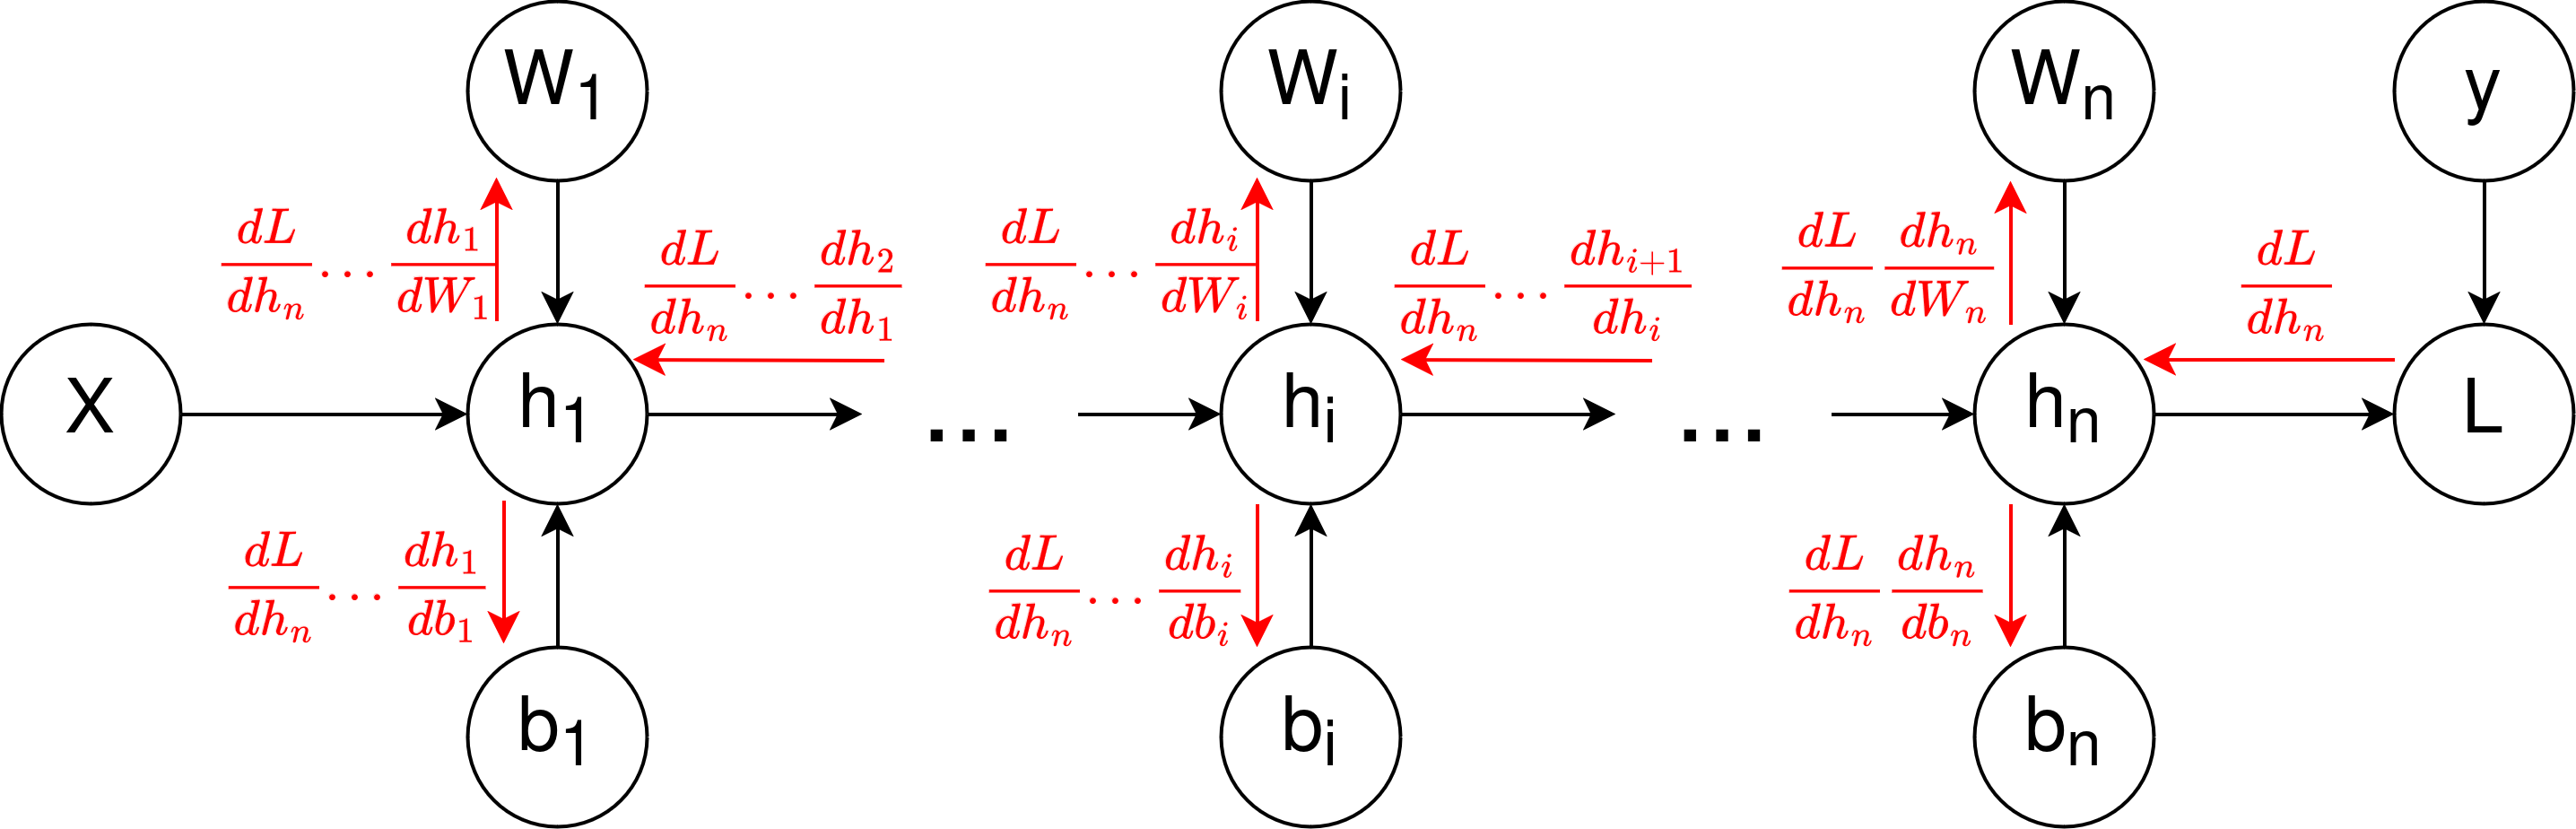
\includegraphics[width=8.5cm]{ANN_back_prop.png}
    \caption{Обратное распространение ошибки по графу вычислений детерминированной полносвязной сети}
    \label{fig:image2}
\end{figure}

Однако детерминированные нейронные сети обладают несколькими проблемами:
\begin{itemize}
    \item Переобучение.
    \item Низкая интерпретируемость.
    \item Завышенная/заниженная уверенность модели в предсказаниях, даже если они неверные.
    \item Низкий уровень откалиброванности модели.
\end{itemize}

Указанные проблемы попытаемся решить с помощью байесовского подхода к нейронным сетям, который
 рассмотрим далее.
\end{document}
